%!TEX TS-program = xelatex
%!TEX encoding = UTF-8

% LaTeX source for the errata of the book ``代数学方法'' in Chinese
% Copyright 2018  李文威 (Wen-Wei Li).
% Permission is granted to copy, distribute and/or modify this
% document under the terms of the Creative Commons
% Attribution 4.0 International (CC BY 4.0)
% http://creativecommons.org/licenses/by/4.0/

% 《代数学方法》卷一勘误表 / 李文威
% 使用自定义的文档类 AJerrata.cls. 自动载入 xeCJK.

\documentclass{AJerrata}

\usepackage{unicode-math}

\usepackage[unicode, colorlinks, psdextra, bookmarksnumbered,
	pdfpagelabels=true,
	pdfauthor={李文威 (Wen-Wei Li)},
	pdftitle={代数学方法卷一勘误},
	pdfkeywords={}
]{hyperref}

\setmainfont[
	BoldFont={texgyretermes-bold.otf},
	ItalicFont={texgyretermes-italic.otf},
	BoldItalicFont={texgyretermes-bolditalic.otf},
	PunctuationSpace=2
]{texgyretermes-regular.otf}

\setsansfont[
	BoldFont=FiraSans-Bold.otf,
	ItalicFont=FiraSans-Italic.otf
]{FiraSans-Regular.otf}

\setCJKmainfont[
	BoldFont=Noto Serif CJK SC Bold
]{Noto Serif CJK SC}

\setCJKsansfont[
	BoldFont=Noto Sans CJK SC Bold
]{Noto Sans CJK SC}

\setCJKfamilyfont{emfont}[
	BoldFont=FandolHei-Regular.otf
]{FandolHei-Regular.otf}	% 强调用的字体

\renewcommand{\em}{\bfseries\CJKfamily{emfont}} % 强调

\setmathfont[
	Extension = .otf,
	math-style= TeX,
]{texgyretermes-math}

\usepackage{mathrsfs}
\usepackage{stmaryrd} \SetSymbolFont{stmry}{bold}{U}{stmry}{m}{n}	% 避免警告 (stmryd 不含粗体故)
% \usepackage{array}
% \usepackage{tikz-cd}  % 使用 TikZ 绘图
\usetikzlibrary{positioning, patterns, calc, matrix, shapes.arrows, shapes.symbols}

\usepackage{myarrows}				% 使用自定义的可伸缩箭头
\usepackage{mycommand}				% 引入自定义的惯用的命令


\title{\bfseries 代数学方法(第一卷)勘误表}
\author{李文威}
\date{\today}

\begin{document}
	\maketitle
	以下页码等信息参照高等教育出版社 2019 年 1 月出版之《代数学方法》第一卷, ISBN: 978-7-04-050725-6. 这些错误将在新版一并改正.

	\begin{Errata}
		\item[第 12 页, 倒数第 8 行]
		\Orig 也可以由稍后的无穷公理保证.
		\Corr 也可以划入稍后的无穷公理.
		\Thx{感谢王东瀚指正.}
		
		\item[第 16 页, 定义 1.2.8]
		\Orig 若传递集 $\alpha$ 对于 $\in$ 构成良序集
		\Corr 若传递集 $\alpha$ 对于 $x < y \stackrel{\text{定义}}{\iff} x \in y$ 成为良序集
		\Thx{感谢王东瀚指正.}
		
		\item[第 16 页, 倒数第 5 行]
		\Orig 于是有 $\gamma \in \gamma$, 这同偏序的反称性矛盾.
		\Corr 于是有 $\gamma \in \gamma$, 亦即在偏序集 $(\alpha, \leq)$ 中 $\gamma < \gamma$, 这同 $<$ 的涵义 ($\leq$ 但 $\neq$) 矛盾.
		\Thx{感谢王东瀚指正.}
		
        \item[第 19 页, 倒数第 5 行]
        \Orig $a_\alpha \notin C_\alpha$
        \Corr $a_\alpha \notin \{ a_\beta \}_{\beta < \alpha}$
        \Thx{感谢胡旻杰指正}

		\item[第 23 页, 第 3--4 行]
		\Orig 真前段 (出现两次)
		\Corr 前段

		\item[第 23 页, 第 5 行]
		\Orig 由于 $\sigma$ 无穷...
		\Corr 由于 $\aleph_\sigma$ 无穷...
		\Thx{感谢王东瀚指正.}

        \item[第 35 页, 倒数第 4 行]
        \Orig $X \in \mathrm{Ob}(\mathcal{C})$
        \Corr $X \in \mathrm{Ob}(\mathcal{C}')$
        \Thx{感谢尹梓僮指正.}

        \item[第 35 页, 第 12 行 (命题 2.2.10 证明)]
        将两个箭头的方向调换.
        \Thx{感谢尹梓僮指正.}

		\item[第 38 页, 第 14 行]
		\Orig{由此导出对象和自然变换的同构概念, 其逆若存在则唯一.}
		\Corr{其逆若存在则唯一, 依此定义何谓对象间或函子间的同构.}
		\Thx{感谢王猷指正.}
		
		\item[第 42 页, 倒数第 2 行]
		\Orig ...同构. $Z(\cdots) \simeq $...
		\Corr ...同构 $Z(\cdots) \simeq$...
		\Thx{感谢王东瀚指正.}
		
        \item[第 47 页, 第 4 行]
        \Orig $A \in \mathcal{C}^\wedge$
        \Corr $A \in \mathrm{Ob}(\mathcal{C}^\wedge)$

		\item[第 49 页, 倒数第 9 行]
		\Orig 由此得到伴随对 $(D^{\mathrm{op}}, D, \varphi)$.
		\Corr 由此得到伴随对 $(D^{\mathrm{op}}, D, \varphi^{-1})$.
		\Thx{感谢王东瀚指正.}

        \item[第 50 也, 第 3 行]
        \Orig $\eta_X$
        \Corr $\eta$
        \Thx{感谢蒋之骏指正}
		
		\item[第 54 页最后] \Corr 图表微调成
		\begin{center}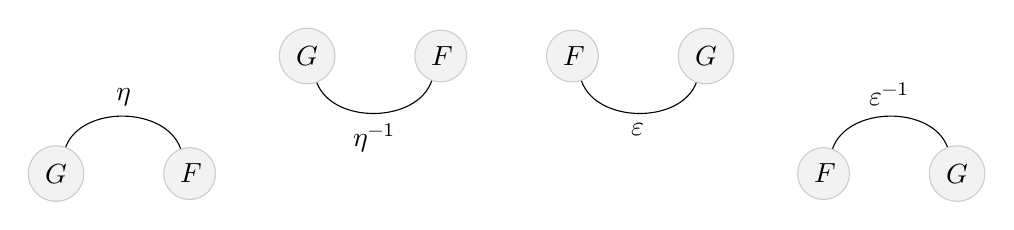
\begin{tikzpicture}[bend angle=70, auto, fct/.style={circle, draw=gray!40, fill=gray!10}]
			\node[fct] (G1) {$G$}; \node[fct] (F1) [right=of G1] {$F$} edge[bend right] node[swap] {$\eta$} (G1);
			\node[fct] (G2) [above right=of F1] {$G$}; \node[fct] (F2) [right=of G2] {$F$} edge[bend left] node {$\eta^{-1}$} (G2);
			\node[fct] (F3) [right=of F2] {$F$}; \node[fct] (G3) [right=of F3] {$G$} edge[bend left] node {$\varepsilon$} (F3);
			\node[fct] (F4) [below right=of G3] {$F$}; \node[fct] (G4) [right=of F4] {$G$} edge[bend right] node[swap] {$\varepsilon^{-1}$} (F4);
		\end{tikzpicture}\end{center}
		兴许更易懂. \Thx{感谢熊锐提供意见.}

        \item[第 94 页, 习题 5 倒数第 2 行]
        \Orig Yang--Baxter 方程.
        \Corr 杨--Baxter 方程.
        
        \item[第 116 页, 第 5 行]
        \Orig $\bar{H} \subseteq N_{\bar{G}}(\bar{H})$
        \Corr $\bar{H} \subsetneq N_{\bar{G}}(\bar{H})$

		\item[第 126 页, 第 6 行]
		\Orig $\left( \cdots \right)_{i=0}^n$
		\Corr $\left( \cdots \right)_{i=0}^{n-1}$

        \item[第 141 页, 第 11 行]
        \Orig 另外约定 $\mathfrak{S}'_n = \{1\}$
        \Corr 另外约定 $\mathfrak{S}'_1 = \{1\}$

		\item[第 149 页, 第 3 行]
		$\mathsf{CRing}$ 表交换环范畴. 另外此行应缩进.
		
		\item[第 156 页, 第 2, 3 行]
		\Orig $a \in R$
		\Corr $a \in I$
		\Thx{感谢阳恩林指正}

		\item[第 165 页, 5.3.11 之上两行]
		\Orig $\exists s \in R$
		\Corr $\exists s \in S$

   		\item[第 205 页, 第 7 行]
		\Orig $M$ 作为 $R/\mathrm{ann}(M)$-模自动是无挠的.
		\Corr $M$ 作为 $R/\mathrm{ann}(M)$-模的零化子自动是 $\{0\}$.
		\Thx{感谢戴懿韡指正.}

        \item[第 218 页, 第 13 行]
        \Orig $B(rx, ys) = rB(x,y)s, \quad r \in R, \; s \in S$.
        \Corr $B(qx, ys) = qB(x,y)s, \quad q \in Q, \; s \in S$.
        \Thx{感谢冯敏立指正.}

        \item[第 220 页]
        本页出现的 $\mathrm{Bil}(\bullet \times \bullet; \bullet)$ 都应该改成 $\mathrm{Bil}(\bullet, \bullet; \bullet)$, 以和 216 页的符号保持一致.
       
        \item[第 228 页, 倒数第 4 行]
        \Orig $\sum_{y \in R}$
        \Corr $\sum_{y \in Y}$
        
        \item[第 230 页, 第 13 行]
        \Orig 萃取处
        \Corr 萃取出
        
		\item[第 230 页, 第 6 行; 第 231 页, 第 9---10 行]
		\Orig $\mathfrak{o}_i$
		\Corr $\mathfrak{d}_i$
		\Thx{感谢郑维喆指正}
        
        \item[第 235 页底部]
        图表中的垂直箭头 $f_i$, $f_{i-1}$ 应改为 $\phi_i$, $\phi_{i-1}$.
        
        \item[第 237 页, 命题 6.8.5 证明最后两行]
        \Orig 故 $(v) \implies (i)$;
        \Corr 故 $(iv) \implies (i)$;
        
        \item[第 238 页, 第 8 行]
        \Orig $Y' \to Y \to Y$ 正合
        \Corr $Y' \to Y \to Y''$ 正合
        
   		\item[第 244 页, 倒数第 10 行]
        \Orig 下面的引理 6.10.4
        \Corr 引理 5.7.4
        \Thx{感谢郑维喆指正}
        
   		\item[第 246 页, 第 2 行和定理 6.10.6, 6.10.7]
		``交换 Noether 模''应改为``交换 Noether 环''. 两个定理的陈述中应该要求 $R$ 是交换 Noether 环.
		\Thx{感谢郑维喆指正}
        
        \item[第 246 頁, 第 16 行]
        \Orig $u_i f_i$
        \Corr $u_i \alpha_i$
        \Thx{感谢陆睿远指正.}
        
        \item[第 247 頁, 第 6---7 行]
        \Orig 其长度记为 $n+1$.
        \Corr 其长度定为 $n$.

  		\item[第 251 页起, 第 6.12 节]
		术语``不可分模''似作``不可分解模''更佳, 以免歧义. (第 4 页倒数第 3 行也应同步修改)
		\Thx{感谢郑维喆指正}

        \item[第 252 頁, 第 2 行]
        \Orig $1 \leq 1 \leq n$.
        \Corr $1 \leq i \leq n$.
        \Thx{感谢傅煌指正.}
        
		\item[第 255 页, 第 1 题]
		\Orig
		\[ N = \lrangle{ \alpha(f)(x_i) - x_j : i \xrightarrow{f} j, \;  x_i \in M_i, x_j \in M_j } \]
		\Corr
		\[ N = \lrangle{ \alpha(f)(x_i) - x_i : i \xrightarrow{f} j, \; x_i \in M_i } \]
		\Thx{感谢郑维喆指正}
        
        \item[第 264 頁, 第 14 行]
        \Orig 如果 $\mathrm{ann}(M) = \{0\}$
        \Corr 如果 $\mathrm{ann}(N) = \{0\}$

        \item[第 274 页, 倒数第 2 行]
        将两处 $A^k(M)$ 改成 $A^k(X)$.
        
		\item[第 284 頁, 定理 7.6.6]
		将定理陈述中的函子 $U$ 由忘却函子改成映 $A$ 为 $A_1$ 的函子, 其余不变. 相应地, 证明第二段的 $\varphi: M \to A$ 应改成 $\varphi: M \to A_1$.
		\Thx{感谢郑维喆指正}
		
		\item[第 285 頁, 倒数第 5 行]
		$T_\chi^n(M) := \left\{ x \in T^n(M) : \forall \sigma \in \mathfrak{S}_n, \; \sigma x = \chi(\sigma) x \right\}$
		\Thx{感谢郑维喆指正}

		\item[第 286 頁, 第 10 行]
		\Orig $\chi = 1, \sigma$
		\Corr $\chi = 1, \sgn$
		
		\item[第 286 頁, 定理 7.6.10]
		原``因而有 $R$-模的同构''改为``因而恒等诱导 $R$-模的同构''. 以下两行公式开头的 $e_1:$ 和 $e_{\sgn}: $ 皆删去.
		\Thx{感谢郑维喆指正}
        
        \item[第 311 页, 命题 8.3.2 证明第 4 行]
        \Corr 分别取......和 $\overline{F}' | E'$.
        
  		\item[第 313 頁, 命题 8.3.9 (iii)]
  		``交''改为``非空交''. 相应地, 证明第四行的``一族正规子扩张''后面加上``且 $I$ 非空''.
        \Thx{感谢郑维喆指正}
        
   		\item[第 315 頁, 定理 8.4.3 (iv)]
        \Orig $\sum_{k \geq 0}^n$
        \Corr $\sum_{k=0}^n$
        \Thx{感谢郑维喆指正}

        \item[第 315 页, 倒数第 2 行]
        \Orig $\deg f(X^p) = pf(X)$
        \Corr $\deg f(X^p) = p \deg f(X)$
        \Thx{感谢杨历指正.}
        
        \item[第 317 页, 倒数第 13 行]
        (出现两次)\;
        \Orig $\prod_{i=1}^n \cdots$
        \Corr $\prod_{m=1}^n \cdots$
        
   		\item[第 348 页, 命题 9.3.6]
        \Orig $\varprojlim_m \Z/n\Z$
        \Corr $\varprojlim_m \Z/m\Z$
        \Thx{感谢郑维喆指正}
        
   		\item[第 352 页, 第 7 行]
        \Orig $p \mid n$
        \Corr $p \nmid n$
        \Thx{感谢郑维喆指正}
        
        \item[第 359 页, 倒数第 2 行]
        \Orig $\in A_F$
        \Corr $\in A_E$
        \Thx{感谢杨历指正.}
        
        \item[第 360 页, 证明]
        将所有 $\chi(\cdots) = 1$ 改成 $\chi(\cdots) = 0$, 以确保与之前的惯例一致.
        \Thx{感谢杨历指正.}
        
   		\item[第 363 页, 倒数第 4 行]
        \Orig $\eta_{[E:F]}$
        \Corr $\eta_{[L:F]}$
        \Thx{感谢郑维喆指正}
        
   		\item[第 372 页, 第 20 题]
        问题 (b) 部分的 $P \in F[X]$ 改成 $Q \in F[X]$, 以免冲突. 相应地, 提示第一段的 $P$ 都改成 $Q$.
        \Thx{感谢郑维喆指正}
        
        \item[第 395--396 页, 引理 10.5.3 的证明]
        从第 395 页倒数第 3 行起 (即证明第二段), 修改如下:

		置 $f_k = \sum_{h \geq 0} c_{k,h} t^h$. 注意到 $\lim_{k \to \infty} \|f_k\| = 0$, 这确保 $c_h := \sum_{k \geq 0} c_{k,h}$ 存在. 我们断言 $f := \sum_{h \geq 0} c_h t^h \in K\lrangle{t}$ 并给出 $\sum_{k=0}^\infty f_k$.
        
        对任意 $\epsilon > 0$, 取 $M$ 充分大使得 $k \geq M \implies \|f_k\| < \epsilon$, 再取 $N$ 使得当 $0 \leq k < M$ 而 $h \geq N$ 时 $|c_{k,h}| < \epsilon$. 于是
        \[ h \geq N \implies \left( \forall k \geq 0, \; |c_{k,h}| \leq \epsilon \right) \implies |c_h| \leq \epsilon, \]
        故 $f := \sum_{h \geq 0} c_h t^h \in K\lrangle{t}$. 其次, 在 $K\lrangle{t}$ 中有等式
        \[ f - \sum_{k=0}^M f_k = \sum_{h \geq 0} \left( c_h - \sum_{k=0}^M c_{k,h} \right) t^h = \sum_{h \geq 0} \underbracket{ \left( \sum_{k > M} c_{k,h} \right)}_{|\cdot| \leq \epsilon} t^h , \]
        从而 $f = \sum_{k=0}^\infty f_k$.
        
        \Thx{感谢高煦指正.}

        \item[第 397 页, 条目 V 下第 6 行]
        \Orig $w_{x.-}$
        \Corr $w_{x,-}$
        
        \item[第 417 页, 最后一行] 它被刻画为对...
	\end{Errata}
\end{document}
